\documentclass{article}
\usepackage{graphicx}
\usepackage{booktabs}
\usepackage{caption}
\usepackage{amsmath}
\usepackage{placeins}
\usepackage{pgfplotstable}
\usepackage{float}

\title{Student Marks Report}
\author{ARNAV MISHRA}
\date{\today}

\begin{document}

\maketitle

\section{Marks Table}
The table below shows the marks obtained by students across various courses.

\begin{table}[h!]
    \centering
    \caption{Marks obtained by students across various courses}
    \pgfplotstabletypeset[
        col sep=space,
        header=true,
        string type,
        every head row/.style={before row=\toprule, after row=\midrule},
        every last row/.style={after row=\bottomrule},
        every row/.style={font=\small},
        columns/0/.style={column name=CourseID},
        columns/1/.style={column name=Student 1},
        columns/2/.style={column name=Student 2},
        columns/3/.style={column name=Student 3},
    ]{marks.dat}
\end{table}

\section{Plots of Marks}
The following figures represent different visualizations of the marks data.

\subsection{Linespoints Plot}
Figure \ref{fig:linespoints} shows the marks for each student plotted using lines and points.

\begin{figure}[H]
    \centering
    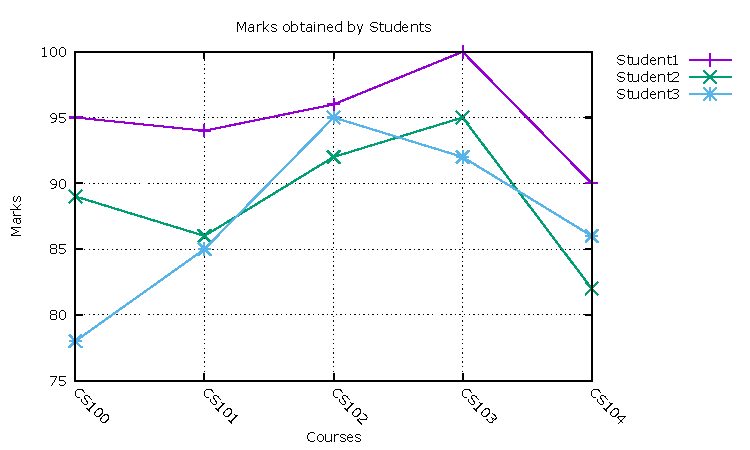
\includegraphics[width=0.8\textwidth]{linespoints.pdf}
    \caption{Marks obtained by students (Linespoints plot)}
    \label{fig:linespoints}
\end{figure}

\subsection{Clustered Histogram}
Figure \ref{fig:histogram} displays a clustered histogram that shows the distribution of marks for each student across the courses.

\begin{figure}[H]
    \centering
    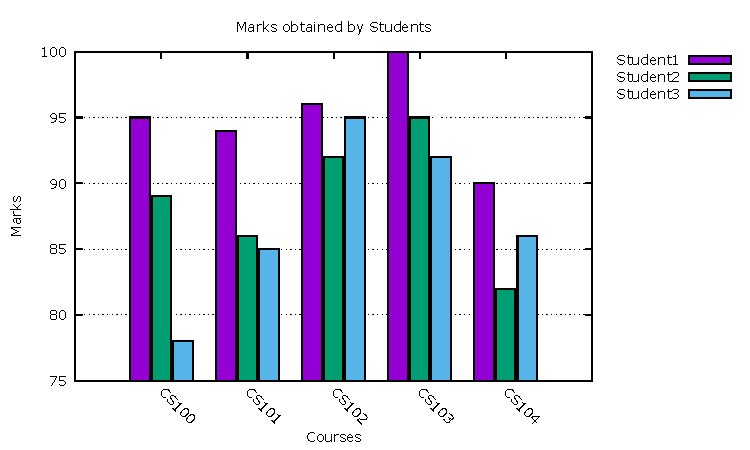
\includegraphics[width=0.8\textwidth]{histogram.pdf}
    \caption{Marks obtained by students (Clustered Histogram)}
    \label{fig:histogram}
\end{figure}

\subsection{Stacked Histogram}
Figure \ref{fig:stacked} presents the same data using a stacked histogram, making it easier to compare the cumulative marks.

\begin{figure}[H]
    \centering
    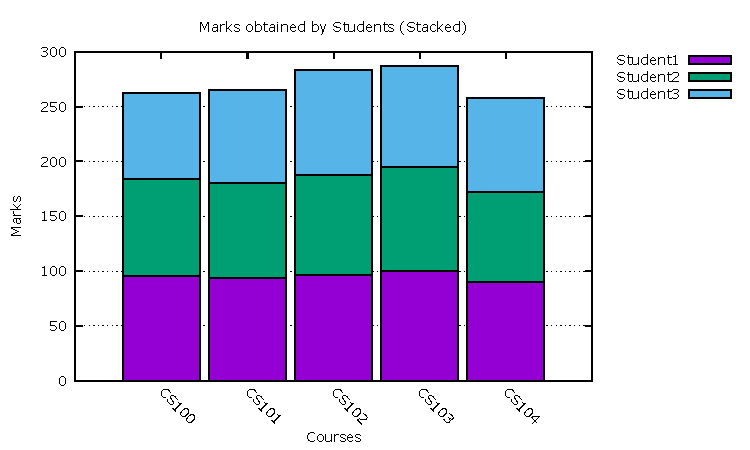
\includegraphics[width=0.8\textwidth]{stacked_histogram.pdf}
    \caption{Marks obtained by students (Stacked Histogram)}
    \label{fig:stacked}
\end{figure}

\FloatBarrier

\section{Discussion}
The plots above provide three different ways to visualize the same data. The linespoints plot (Figure \ref{fig:linespoints}) shows individual student performance across courses. The clustered histogram (Figure \ref{fig:histogram}) gives a side-by-side comparison of each student's marks, while the stacked histogram (Figure \ref{fig:stacked}) highlights the combined totals for each course.

\end{document}

